\documentclass[1p]{elsarticle_modified}
%\bibliographystyle{elsarticle-num}

%\usepackage[colorlinks]{hyperref}
%\usepackage{abbrmath_seonhwa} %\Abb, \Ascr, \Acal ,\Abf, \Afrak
\usepackage{amsfonts}
\usepackage{amssymb}
\usepackage{amsmath}
\usepackage{amsthm}
\usepackage{scalefnt}
\usepackage{amsbsy}
\usepackage{kotex}
\usepackage{caption}
\usepackage{subfig}
\usepackage{color}
\usepackage{graphicx}
\usepackage{xcolor} %% white, black, red, green, blue, cyan, magenta, yellow
\usepackage{float}
\usepackage{setspace}
\usepackage{hyperref}

\usepackage{tikz}
\usetikzlibrary{arrows}

\usepackage{multirow}
\usepackage{array} % fixed length table
\usepackage{hhline}

%%%%%%%%%%%%%%%%%%%%%
\makeatletter
\renewcommand*\env@matrix[1][\arraystretch]{%
	\edef\arraystretch{#1}%
	\hskip -\arraycolsep
	\let\@ifnextchar\new@ifnextchar
	\array{*\c@MaxMatrixCols c}}
\makeatother %https://tex.stackexchange.com/questions/14071/how-can-i-increase-the-line-spacing-in-a-matrix
%%%%%%%%%%%%%%%

\usepackage[normalem]{ulem}

\newcommand{\msout}[1]{\ifmmode\text{\sout{\ensuremath{#1}}}\else\sout{#1}\fi}
%SOURCE: \msout is \stkout macro in https://tex.stackexchange.com/questions/20609/strikeout-in-math-mode

\newcommand{\cancel}[1]{
	\ifmmode
	{\color{red}\msout{#1}}
	\else
	{\color{red}\sout{#1}}
	\fi
}

\newcommand{\add}[1]{
	{\color{blue}\uwave{#1}}
}

\newcommand{\replace}[2]{
	\ifmmode
	{\color{red}\msout{#1}}{\color{blue}\uwave{#2}}
	\else
	{\color{red}\sout{#1}}{\color{blue}\uwave{#2}}
	\fi
}

\newcommand{\Sol}{\mathcal{S}} %segment
\newcommand{\D}{D} %diagram
\newcommand{\A}{\mathcal{A}} %arc


%%%%%%%%%%%%%%%%%%%%%%%%%%%%%5 test

\def\sl{\operatorname{\textup{SL}}(2,\Cbb)}
\def\psl{\operatorname{\textup{PSL}}(2,\Cbb)}
\def\quan{\mkern 1mu \triangleright \mkern 1mu}

\theoremstyle{definition}
\newtheorem{thm}{Theorem}[section]
\newtheorem{prop}[thm]{Proposition}
\newtheorem{lem}[thm]{Lemma}
\newtheorem{ques}[thm]{Question}
\newtheorem{cor}[thm]{Corollary}
\newtheorem{defn}[thm]{Definition}
\newtheorem{exam}[thm]{Example}
\newtheorem{rmk}[thm]{Remark}
\newtheorem{alg}[thm]{Algorithm}

\newcommand{\I}{\sqrt{-1}}
\begin{document}

%\begin{frontmatter}
%
%\title{Boundary parabolic representations of knots up to 8 crossings}
%
%%% Group authors per affiliation:
%\author{Yunhi Cho} 
%\address{Department of Mathematics, University of Seoul, Seoul, Korea}
%\ead{yhcho@uos.ac.kr}
%
%
%\author{Seonhwa Kim} %\fnref{s_kim}}
%\address{Center for Geometry and Physics, Institute for Basic Science, Pohang, 37673, Korea}
%\ead{ryeona17@ibs.re.kr}
%
%\author{Hyuk Kim}
%\address{Department of Mathematical Sciences, Seoul National University, Seoul 08826, Korea}
%\ead{hyukkim@snu.ac.kr}
%
%\author{Seokbeom Yoon}
%\address{Department of Mathematical Sciences, Seoul National University, Seoul, 08826,  Korea}
%\ead{sbyoon15@snu.ac.kr}
%
%\begin{abstract}
%We find all boundary parabolic representation of knots up to 8 crossings.
%
%\end{abstract}
%\begin{keyword}
%    \MSC[2010] 57M25 
%\end{keyword}
%
%\end{frontmatter}

%\linenumbers
%\tableofcontents
%
\newcommand\colored[1]{\textcolor{white}{\rule[-0.35ex]{0.8em}{1.4ex}}\kern-0.8em\color{red} #1}%
%\newcommand\colored[1]{\textcolor{white}{ #1}\kern-2.17ex	\textcolor{white}{ #1}\kern-1.81ex	\textcolor{white}{ #1}\kern-2.15ex\color{red}#1	}

{\Large $\underline{12n_{0333}~(K12n_{0333})}$}

\setlength{\tabcolsep}{10pt}
\renewcommand{\arraystretch}{1.6}
\vspace{1cm}\begin{tabular}{m{100pt}>{\centering\arraybackslash}m{274pt}}
\multirow{5}{120pt}{
	\centering
	\includegraphics[width=112pt]{../../../GIT/diagram.site/Diagrams/png/2422_12n_0333.png}\\
\ \ \ A knot diagram\footnotemark}&
\allowdisplaybreaks
\textbf{Linearized knot diagam} \\
\cline{2-2}
 &
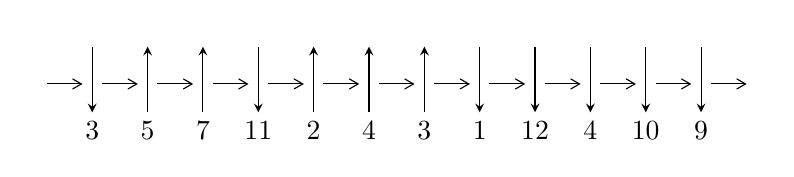
\begin{tikzpicture}[x=20pt, y=17pt]
	% nodes
	\node (C0) at (0, 0) {};
	\node (C1) at (1, 0) {};
	\node (C1U) at (1, +1) {};
	\node (C1D) at (1, -1) {3};

	\node (C2) at (2, 0) {};
	\node (C2U) at (2, +1) {};
	\node (C2D) at (2, -1) {5};

	\node (C3) at (3, 0) {};
	\node (C3U) at (3, +1) {};
	\node (C3D) at (3, -1) {7};

	\node (C4) at (4, 0) {};
	\node (C4U) at (4, +1) {};
	\node (C4D) at (4, -1) {11};

	\node (C5) at (5, 0) {};
	\node (C5U) at (5, +1) {};
	\node (C5D) at (5, -1) {2};

	\node (C6) at (6, 0) {};
	\node (C6U) at (6, +1) {};
	\node (C6D) at (6, -1) {4};

	\node (C7) at (7, 0) {};
	\node (C7U) at (7, +1) {};
	\node (C7D) at (7, -1) {3};

	\node (C8) at (8, 0) {};
	\node (C8U) at (8, +1) {};
	\node (C8D) at (8, -1) {1};

	\node (C9) at (9, 0) {};
	\node (C9U) at (9, +1) {};
	\node (C9D) at (9, -1) {12};

	\node (C10) at (10, 0) {};
	\node (C10U) at (10, +1) {};
	\node (C10D) at (10, -1) {4};

	\node (C11) at (11, 0) {};
	\node (C11U) at (11, +1) {};
	\node (C11D) at (11, -1) {10};

	\node (C12) at (12, 0) {};
	\node (C12U) at (12, +1) {};
	\node (C12D) at (12, -1) {9};
	\node (C13) at (13, 0) {};

	% arrows
	\draw[->,>={angle 60}]
	(C0) edge (C1) (C1) edge (C2) (C2) edge (C3) (C3) edge (C4) (C4) edge (C5) (C5) edge (C6) (C6) edge (C7) (C7) edge (C8) (C8) edge (C9) (C9) edge (C10) (C10) edge (C11) (C11) edge (C12) (C12) edge (C13) ;	\draw[->,>=stealth]
	(C1U) edge (C1D) (C2D) edge (C2U) (C3D) edge (C3U) (C4U) edge (C4D) (C5D) edge (C5U) (C6D) edge (C6U) (C7D) edge (C7U) (C8U) edge (C8D) (C9U) edge (C9D) (C10U) edge (C10D) (C11U) edge (C11D) (C12U) edge (C12D) ;
	\end{tikzpicture} \\
\hhline{~~} \\& 
\textbf{Solving Sequence} \\ \cline{2-2} 
 &
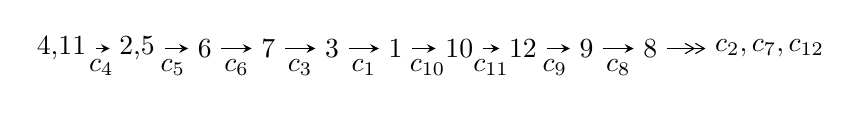
\begin{tikzpicture}[x=23pt, y=7pt]
	% node
	\node (A0) at (-1/8, 0) {4,11};
	\node (A1) at (17/16, 0) {2,5};
	\node (A2) at (17/8, 0) {6};
	\node (A3) at (25/8, 0) {7};
	\node (A4) at (33/8, 0) {3};
	\node (A5) at (41/8, 0) {1};
	\node (A6) at (49/8, 0) {10};
	\node (A7) at (57/8, 0) {12};
	\node (A8) at (65/8, 0) {9};
	\node (A9) at (73/8, 0) {8};
	\node (C1) at (1/2, -1) {$c_{4}$};
	\node (C2) at (13/8, -1) {$c_{5}$};
	\node (C3) at (21/8, -1) {$c_{6}$};
	\node (C4) at (29/8, -1) {$c_{3}$};
	\node (C5) at (37/8, -1) {$c_{1}$};
	\node (C6) at (45/8, -1) {$c_{10}$};
	\node (C7) at (53/8, -1) {$c_{11}$};
	\node (C8) at (61/8, -1) {$c_{9}$};
	\node (C9) at (69/8, -1) {$c_{8}$};
	\node (A10) at (11, 0) {$c_{2},c_{7},c_{12}$};

	% edge
	\draw[->,>=stealth]	
	(A0) edge (A1) (A1) edge (A2) (A2) edge (A3) (A3) edge (A4) (A4) edge (A5) (A5) edge (A6) (A6) edge (A7) (A7) edge (A8) (A8) edge (A9) ;
	\draw[->>,>={angle 60}]	
	(A9) edge (A10);
\end{tikzpicture} \\ 

\end{tabular} \\

\footnotetext{
The image of knot diagram is generated by the software ``\textbf{Draw programme}" developed by Andrew Bartholomew(\url{http://www.layer8.co.uk/maths/draw/index.htm\#Running-draw}), where we modified some parts for our purpose(\url{https://github.com/CATsTAILs/LinksPainter}).
}\phantom \\ \newline 
\centering \textbf{Ideals for irreducible components\footnotemark of $X_{\text{par}}$} 
 
\begin{align*}
I^u_{1}&=\langle 
u^{14}- u^{13}- u^{12}+3 u^{11}+3 u^{10}-5 u^9-2 u^8+7 u^7+3 u^6-6 u^5-2 u^4+4 u^3+b- u+1,\\
\phantom{I^u_{1}}&\phantom{= \langle  }- u^{15}+u^{14}+u^{13}-2 u^{12}-3 u^{11}+4 u^{10}+4 u^9-4 u^8-3 u^7+4 u^6+6 u^5-2 u^4+2 a-1,\\
\phantom{I^u_{1}}&\phantom{= \langle  }u^{16}-3 u^{15}+3 u^{14}+2 u^{13}-3 u^{12}-6 u^{11}+12 u^{10}-9 u^8-2 u^7+12 u^6-2 u^5-8 u^4+4 u^3+2 u^2-3 u+2\rangle \\
I^u_{2}&=\langle 
b+1,\;2 u^5 a+4 u^6+2 u^4 a+7 u^5+3 u^4-2 u^2 a-2 u^3+a^2+4 a u+7 u^2+3 a+14 u+5,\\
\phantom{I^u_{2}}&\phantom{= \langle  }u^7+u^6- u^4+2 u^3+2 u^2-1\rangle \\
I^u_{3}&=\langle 
u^7- u^5+2 u^3+b- u+1,\;u^7- u^6+u^5+u^4+2 u^3-3 u^2+a+2 u+2,\;u^8- u^6+3 u^4-2 u^2+1\rangle \\
\\
\end{align*}
\raggedright * 3 irreducible components of $\dim_{\mathbb{C}}=0$, with total 38 representations.\\
\footnotetext{All coefficients of polynomials are rational numbers. But the coefficients are sometimes approximated in decimal forms when there is not enough margin.}
\newpage
\renewcommand{\arraystretch}{1}
\centering \section*{I. $I^u_{1}= \langle u^{14}- u^{13}+\cdots+b+1,\;- u^{15}+u^{14}+\cdots+2 a-1,\;u^{16}-3 u^{15}+\cdots-3 u+2 \rangle$}
\flushleft \textbf{(i) Arc colorings}\\
\begin{tabular}{m{7pt} m{180pt} m{7pt} m{180pt} }
\flushright $a_{4}=$&$\begin{pmatrix}1\\0\end{pmatrix}$ \\
\flushright $a_{11}=$&$\begin{pmatrix}0\\u\end{pmatrix}$ \\
\flushright $a_{2}=$&$\begin{pmatrix}\frac{1}{2} u^{15}-\frac{1}{2} u^{14}+\cdots+u^4+\frac{1}{2}\\- u^{14}+u^{13}+\cdots+u-1\end{pmatrix}$ \\
\flushright $a_{5}=$&$\begin{pmatrix}1\\u^2\end{pmatrix}$ \\
\flushright $a_{6}=$&$\begin{pmatrix}-\frac{1}{2} u^{15}+\frac{3}{2} u^{14}+\cdots- u+\frac{3}{2}\\u^{15}-2 u^{14}+3 u^{12}+u^{11}-7 u^{10}+u^9+6 u^8-7 u^6+4 u^4- u^3+u-1\end{pmatrix}$ \\
\flushright $a_{7}=$&$\begin{pmatrix}\frac{1}{2} u^{15}-\frac{1}{2} u^{14}+\cdots+u^4+\frac{1}{2}\\u^{15}-2 u^{14}+3 u^{12}+u^{11}-7 u^{10}+u^9+6 u^8-7 u^6+4 u^4- u^3+u-1\end{pmatrix}$ \\
\flushright $a_{3}=$&$\begin{pmatrix}-\frac{1}{2} u^{15}+\frac{3}{2} u^{14}+\cdots- u+\frac{3}{2}\\u^{14}- u^{13}+\cdots+u^3+1\end{pmatrix}$ \\
\flushright $a_{1}=$&$\begin{pmatrix}- u^7-2 u^3\\- u^7+u^5-2 u^3+u\end{pmatrix}$ \\
\flushright $a_{10}=$&$\begin{pmatrix}u\\u\end{pmatrix}$ \\
\flushright $a_{12}=$&$\begin{pmatrix}- u^3\\- u^3+u\end{pmatrix}$ \\
\flushright $a_{9}=$&$\begin{pmatrix}u^5+u\\u^5- u^3+u\end{pmatrix}$ \\
\flushright $a_{8}=$&$\begin{pmatrix}u^9+3 u^5+u\\u^9- u^7+3 u^5-2 u^3+u\end{pmatrix}$\\&\end{tabular}
\flushleft \textbf{(ii) Obstruction class $= -1$}\\~\\
\flushleft \textbf{(iii) Cusp Shapes $= 2 u^{15}-4 u^{14}+10 u^{12}-18 u^{10}+10 u^9+24 u^8-8 u^7-22 u^6+12 u^5+20 u^4-8 u^3-8 u^2+6 u-2$}\\~\\
\newpage\renewcommand{\arraystretch}{1}
\flushleft \textbf{(iv) u-Polynomials at the component}\newline \\
\begin{tabular}{m{50pt}|m{274pt}}
Crossings & \hspace{64pt}u-Polynomials at each crossing \\
\hline $$\begin{aligned}c_{1}\end{aligned}$$&$\begin{aligned}
&u^{16}+2 u^{15}+\cdots+7 u+1
\end{aligned}$\\
\hline $$\begin{aligned}c_{2},c_{3},c_{5}\\c_{6},c_{7}\end{aligned}$$&$\begin{aligned}
&u^{16}+u^{14}+\cdots+u+1
\end{aligned}$\\
\hline $$\begin{aligned}c_{4},c_{10}\end{aligned}$$&$\begin{aligned}
&u^{16}-3 u^{15}+\cdots-3 u+2
\end{aligned}$\\
\hline $$\begin{aligned}c_{8},c_{9},c_{11}\\c_{12}\end{aligned}$$&$\begin{aligned}
&u^{16}+3 u^{15}+\cdots+u+4
\end{aligned}$\\
\hline
\end{tabular}\\~\\
\newpage\renewcommand{\arraystretch}{1}
\flushleft \textbf{(v) Riley Polynomials at the component}\newline \\
\begin{tabular}{m{50pt}|m{274pt}}
Crossings & \hspace{64pt}Riley Polynomials at each crossing \\
\hline $$\begin{aligned}c_{1}\end{aligned}$$&$\begin{aligned}
&y^{16}+34 y^{15}+\cdots+3 y+1
\end{aligned}$\\
\hline $$\begin{aligned}c_{2},c_{3},c_{5}\\c_{6},c_{7}\end{aligned}$$&$\begin{aligned}
&y^{16}+2 y^{15}+\cdots+7 y+1
\end{aligned}$\\
\hline $$\begin{aligned}c_{4},c_{10}\end{aligned}$$&$\begin{aligned}
&y^{16}-3 y^{15}+\cdots- y+4
\end{aligned}$\\
\hline $$\begin{aligned}c_{8},c_{9},c_{11}\\c_{12}\end{aligned}$$&$\begin{aligned}
&y^{16}+21 y^{15}+\cdots-33 y+16
\end{aligned}$\\
\hline
\end{tabular}\\~\\
\newpage\flushleft \textbf{(vi) Complex Volumes and Cusp Shapes}
$$\begin{array}{c|c|c}  
\text{Solutions to }I^u_{1}& \I (\text{vol} + \sqrt{-1}CS) & \text{Cusp shape}\\
 \hline 
\begin{aligned}
u &= \phantom{-}0.928405 + 0.260033 I \\
a &= \phantom{-}0.35481 - 2.30363 I \\
b &= \phantom{-}0.773479 - 1.013430 I\end{aligned}
 & -1.18138 - 3.90571 I & -4.06432 + 8.02120 I \\ \hline\begin{aligned}
u &= \phantom{-}0.928405 - 0.260033 I \\
a &= \phantom{-}0.35481 + 2.30363 I \\
b &= \phantom{-}0.773479 + 1.013430 I\end{aligned}
 & -1.18138 + 3.90571 I & -4.06432 - 8.02120 I \\ \hline\begin{aligned}
u &= -0.650391 + 0.833172 I \\
a &= -0.136050 + 0.366350 I \\
b &= \phantom{-}1.39607 - 0.78392 I\end{aligned}
 & \phantom{-}5.41244 - 2.99211 I & \phantom{-}2.13069 + 2.15940 I \\ \hline\begin{aligned}
u &= -0.650391 - 0.833172 I \\
a &= -0.136050 - 0.366350 I \\
b &= \phantom{-}1.39607 + 0.78392 I\end{aligned}
 & \phantom{-}5.41244 + 2.99211 I & \phantom{-}2.13069 - 2.15940 I \\ \hline\begin{aligned}
u &= -0.816725 + 0.248973 I \\
a &= \phantom{-}0.91106 - 1.21568 I \\
b &= -0.198116 - 0.632117 I\end{aligned}
 & -1.43484 + 0.76137 I & -4.76909 - 0.41867 I \\ \hline\begin{aligned}
u &= -0.816725 - 0.248973 I \\
a &= \phantom{-}0.91106 + 1.21568 I \\
b &= -0.198116 + 0.632117 I\end{aligned}
 & -1.43484 - 0.76137 I & -4.76909 + 0.41867 I \\ \hline\begin{aligned}
u &= -0.970812 + 0.659855 I \\
a &= -0.66898 + 2.08400 I \\
b &= \phantom{-}1.47947 + 0.97775 I\end{aligned}
 & \phantom{-}4.31472 + 8.49137 I & -0.41000 - 7.95274 I \\ \hline\begin{aligned}
u &= -0.970812 - 0.659855 I \\
a &= -0.66898 - 2.08400 I \\
b &= \phantom{-}1.47947 - 0.97775 I\end{aligned}
 & \phantom{-}4.31472 - 8.49137 I & -0.41000 + 7.95274 I \\ \hline\begin{aligned}
u &= \phantom{-}0.905631 + 0.833459 I \\
a &= \phantom{-}0.431652 + 0.930570 I \\
b &= -1.368560 + 0.130086 I\end{aligned}
 & \phantom{-}4.87488 - 3.10725 I & \phantom{-}2.83461 + 2.27885 I \\ \hline\begin{aligned}
u &= \phantom{-}0.905631 - 0.833459 I \\
a &= \phantom{-}0.431652 - 0.930570 I \\
b &= -1.368560 - 0.130086 I\end{aligned}
 & \phantom{-}4.87488 + 3.10725 I & \phantom{-}2.83461 - 2.27885 I\\
 \hline 
 \end{array}$$\newpage$$\begin{array}{c|c|c}  
\text{Solutions to }I^u_{1}& \I (\text{vol} + \sqrt{-1}CS) & \text{Cusp shape}\\
 \hline 
\begin{aligned}
u &= \phantom{-}0.915125 + 0.963980 I \\
a &= -0.269698 - 0.434629 I \\
b &= \phantom{-}1.81390 + 0.76762 I\end{aligned}
 & \phantom{-}15.6936 + 4.6465 I & \phantom{-}1.09085 - 1.72729 I \\ \hline\begin{aligned}
u &= \phantom{-}0.915125 - 0.963980 I \\
a &= -0.269698 + 0.434629 I \\
b &= \phantom{-}1.81390 - 0.76762 I\end{aligned}
 & \phantom{-}15.6936 - 4.6465 I & \phantom{-}1.09085 + 1.72729 I \\ \hline\begin{aligned}
u &= \phantom{-}0.993185 + 0.916284 I \\
a &= -0.97982 - 1.63330 I \\
b &= \phantom{-}1.84398 - 0.79885 I\end{aligned}
 & \phantom{-}15.4310 - 11.5459 I & \phantom{-}0.63569 + 6.14734 I \\ \hline\begin{aligned}
u &= \phantom{-}0.993185 - 0.916284 I \\
a &= -0.97982 + 1.63330 I \\
b &= \phantom{-}1.84398 + 0.79885 I\end{aligned}
 & \phantom{-}15.4310 + 11.5459 I & \phantom{-}0.63569 - 6.14734 I \\ \hline\begin{aligned}
u &= \phantom{-}0.195584 + 0.595042 I \\
a &= \phantom{-}0.107025 - 0.207653 I \\
b &= \phantom{-}0.759770 + 0.417859 I\end{aligned}
 & \phantom{-}1.30282 + 0.89270 I & \phantom{-}4.55158 - 1.98152 I \\ \hline\begin{aligned}
u &= \phantom{-}0.195584 - 0.595042 I \\
a &= \phantom{-}0.107025 + 0.207653 I \\
b &= \phantom{-}0.759770 - 0.417859 I\end{aligned}
 & \phantom{-}1.30282 - 0.89270 I & \phantom{-}4.55158 + 1.98152 I\\
 \hline 
 \end{array}$$\newpage\newpage\renewcommand{\arraystretch}{1}
\centering \section*{II. $I^u_{2}= \langle b+1,\;2 u^5 a+4 u^6+\cdots+3 a+5,\;u^7+u^6- u^4+2 u^3+2 u^2-1 \rangle$}
\flushleft \textbf{(i) Arc colorings}\\
\begin{tabular}{m{7pt} m{180pt} m{7pt} m{180pt} }
\flushright $a_{4}=$&$\begin{pmatrix}1\\0\end{pmatrix}$ \\
\flushright $a_{11}=$&$\begin{pmatrix}0\\u\end{pmatrix}$ \\
\flushright $a_{2}=$&$\begin{pmatrix}a\\-1\end{pmatrix}$ \\
\flushright $a_{5}=$&$\begin{pmatrix}1\\u^2\end{pmatrix}$ \\
\flushright $a_{6}=$&$\begin{pmatrix}-2 u^5-2 u^4+u^2 a+u^2- a-4 u-2\\- u^2 a+u^2-1\end{pmatrix}$ \\
\flushright $a_{7}=$&$\begin{pmatrix}-2 u^5-2 u^4+2 u^2- a-4 u-3\\- u^2 a+u^2-1\end{pmatrix}$ \\
\flushright $a_{3}=$&$\begin{pmatrix}- u^2 a+a-1\\- u^4 a- u^2-1\end{pmatrix}$ \\
\flushright $a_{1}=$&$\begin{pmatrix}u^6- u^4+2 u^2-1\\u^6+u^5- u^4+2 u^2+u-1\end{pmatrix}$ \\
\flushright $a_{10}=$&$\begin{pmatrix}u\\u\end{pmatrix}$ \\
\flushright $a_{12}=$&$\begin{pmatrix}- u^3\\- u^3+u\end{pmatrix}$ \\
\flushright $a_{9}=$&$\begin{pmatrix}u^5+u\\u^5- u^3+u\end{pmatrix}$ \\
\flushright $a_{8}=$&$\begin{pmatrix}u^4- u^2+1\\u^6+u^2\end{pmatrix}$\\&\end{tabular}
\flushleft \textbf{(ii) Obstruction class $= -1$}\\~\\
\flushleft \textbf{(iii) Cusp Shapes $= -4 u^5-4 u^4+4 u^2-8 u-6$}\\~\\
\newpage\renewcommand{\arraystretch}{1}
\flushleft \textbf{(iv) u-Polynomials at the component}\newline \\
\begin{tabular}{m{50pt}|m{274pt}}
Crossings & \hspace{64pt}u-Polynomials at each crossing \\
\hline $$\begin{aligned}c_{1}\end{aligned}$$&$\begin{aligned}
&u^{14}+3 u^{13}+\cdots+27 u+4
\end{aligned}$\\
\hline $$\begin{aligned}c_{2},c_{3},c_{5}\\c_{6},c_{7}\end{aligned}$$&$\begin{aligned}
&u^{14}+u^{13}+\cdots+5 u+2
\end{aligned}$\\
\hline $$\begin{aligned}c_{4},c_{10}\end{aligned}$$&$\begin{aligned}
&(u^7+u^6- u^4+2 u^3+2 u^2-1)^2
\end{aligned}$\\
\hline $$\begin{aligned}c_{8},c_{9},c_{11}\\c_{12}\end{aligned}$$&$\begin{aligned}
&(u^7+u^6+6 u^5+5 u^4+10 u^3+6 u^2+4 u+1)^2
\end{aligned}$\\
\hline
\end{tabular}\\~\\
\newpage\renewcommand{\arraystretch}{1}
\flushleft \textbf{(v) Riley Polynomials at the component}\newline \\
\begin{tabular}{m{50pt}|m{274pt}}
Crossings & \hspace{64pt}Riley Polynomials at each crossing \\
\hline $$\begin{aligned}c_{1}\end{aligned}$$&$\begin{aligned}
&y^{14}+15 y^{13}+\cdots+95 y+16
\end{aligned}$\\
\hline $$\begin{aligned}c_{2},c_{3},c_{5}\\c_{6},c_{7}\end{aligned}$$&$\begin{aligned}
&y^{14}+3 y^{13}+\cdots+27 y+4
\end{aligned}$\\
\hline $$\begin{aligned}c_{4},c_{10}\end{aligned}$$&$\begin{aligned}
&(y^7- y^6+6 y^5-5 y^4+10 y^3-6 y^2+4 y-1)^2
\end{aligned}$\\
\hline $$\begin{aligned}c_{8},c_{9},c_{11}\\c_{12}\end{aligned}$$&$\begin{aligned}
&(y^7+11 y^6+46 y^5+91 y^4+86 y^3+34 y^2+4 y-1)^2
\end{aligned}$\\
\hline
\end{tabular}\\~\\
\newpage\flushleft \textbf{(vi) Complex Volumes and Cusp Shapes}
$$\begin{array}{c|c|c}  
\text{Solutions to }I^u_{2}& \I (\text{vol} + \sqrt{-1}CS) & \text{Cusp shape}\\
 \hline 
\begin{aligned}
u &= \phantom{-}0.850452 + 0.793787 I \\
a &= \phantom{-}0.529865 + 1.201600 I \\
b &= -1.00000\phantom{ +0.000000I}\end{aligned}
 & \phantom{-}4.70993 - 2.92126 I & \phantom{-}1.79653 + 2.94858 I \\ \hline\begin{aligned}
u &= \phantom{-}0.850452 + 0.793787 I \\
a &= \phantom{-}0.368398 + 0.272687 I \\
b &= -1.00000\phantom{ +0.000000I}\end{aligned}
 & \phantom{-}4.70993 - 2.92126 I & \phantom{-}1.79653 + 2.94858 I \\ \hline\begin{aligned}
u &= \phantom{-}0.850452 - 0.793787 I \\
a &= \phantom{-}0.529865 - 1.201600 I \\
b &= -1.00000\phantom{ +0.000000I}\end{aligned}
 & \phantom{-}4.70993 + 2.92126 I & \phantom{-}1.79653 - 2.94858 I \\ \hline\begin{aligned}
u &= \phantom{-}0.850452 - 0.793787 I \\
a &= \phantom{-}0.368398 - 0.272687 I \\
b &= -1.00000\phantom{ +0.000000I}\end{aligned}
 & \phantom{-}4.70993 + 2.92126 I & \phantom{-}1.79653 - 2.94858 I \\ \hline\begin{aligned}
u &= -0.676751 + 0.491075 I \\
a &= -1.041030 - 0.810129 I \\
b &= -1.00000\phantom{ +0.000000I}\end{aligned}
 & -2.02205 + 1.83261 I & \phantom{-}0.22558 - 5.43914 I \\ \hline\begin{aligned}
u &= -0.676751 + 0.491075 I \\
a &= \phantom{-}1.15382 - 1.90944 I \\
b &= -1.00000\phantom{ +0.000000I}\end{aligned}
 & -2.02205 + 1.83261 I & \phantom{-}0.22558 - 5.43914 I \\ \hline\begin{aligned}
u &= -0.676751 - 0.491075 I \\
a &= -1.041030 + 0.810129 I \\
b &= -1.00000\phantom{ +0.000000I}\end{aligned}
 & -2.02205 - 1.83261 I & \phantom{-}0.22558 + 5.43914 I \\ \hline\begin{aligned}
u &= -0.676751 - 0.491075 I \\
a &= \phantom{-}1.15382 + 1.90944 I \\
b &= -1.00000\phantom{ +0.000000I}\end{aligned}
 & -2.02205 - 1.83261 I & \phantom{-}0.22558 + 5.43914 I \\ \hline\begin{aligned}
u &= -0.962510 + 0.950397 I \\
a &= \phantom{-}0.498708 - 1.218380 I \\
b &= -1.00000\phantom{ +0.000000I}\end{aligned}
 & \phantom{-}16.6015 + 3.4867 I & \phantom{-}1.97231 - 2.18600 I \\ \hline\begin{aligned}
u &= -0.962510 + 0.950397 I \\
a &= \phantom{-}0.487449 + 0.125376 I \\
b &= -1.00000\phantom{ +0.000000I}\end{aligned}
 & \phantom{-}16.6015 + 3.4867 I & \phantom{-}1.97231 - 2.18600 I\\
 \hline 
 \end{array}$$\newpage$$\begin{array}{c|c|c}  
\text{Solutions to }I^u_{2}& \I (\text{vol} + \sqrt{-1}CS) & \text{Cusp shape}\\
 \hline 
\begin{aligned}
u &= -0.962510 - 0.950397 I \\
a &= \phantom{-}0.498708 + 1.218380 I \\
b &= -1.00000\phantom{ +0.000000I}\end{aligned}
 & \phantom{-}16.6015 - 3.4867 I & \phantom{-}1.97231 + 2.18600 I \\ \hline\begin{aligned}
u &= -0.962510 - 0.950397 I \\
a &= \phantom{-}0.487449 - 0.125376 I \\
b &= -1.00000\phantom{ +0.000000I}\end{aligned}
 & \phantom{-}16.6015 - 3.4867 I & \phantom{-}1.97231 + 2.18600 I \\ \hline\begin{aligned}
u &= \phantom{-}0.577619\phantom{ +0.000000I} \\
a &= -2.49721 + 3.11982 I \\
b &= -1.00000\phantom{ +0.000000I}\end{aligned}
 & -4.03510\phantom{ +0.000000I} & -9.98880\phantom{ +0.000000I} \\ \hline\begin{aligned}
u &= \phantom{-}0.577619\phantom{ +0.000000I} \\
a &= -2.49721 - 3.11982 I \\
b &= -1.00000\phantom{ +0.000000I}\end{aligned}
 & -4.03510\phantom{ +0.000000I} & -9.98880\phantom{ +0.000000I}\\
 \hline 
 \end{array}$$\newpage\newpage\renewcommand{\arraystretch}{1}
\centering \section*{III. $I^u_{3}= \langle u^7- u^5+2 u^3+b- u+1,\;u^7- u^6+u^5+u^4+2 u^3-3 u^2+a+2 u+2,\;u^8- u^6+3 u^4-2 u^2+1 \rangle$}
\flushleft \textbf{(i) Arc colorings}\\
\begin{tabular}{m{7pt} m{180pt} m{7pt} m{180pt} }
\flushright $a_{4}=$&$\begin{pmatrix}1\\0\end{pmatrix}$ \\
\flushright $a_{11}=$&$\begin{pmatrix}0\\u\end{pmatrix}$ \\
\flushright $a_{2}=$&$\begin{pmatrix}- u^7+u^6- u^5- u^4-2 u^3+3 u^2-2 u-2\\- u^7+u^5-2 u^3+u-1\end{pmatrix}$ \\
\flushright $a_{5}=$&$\begin{pmatrix}1\\u^2\end{pmatrix}$ \\
\flushright $a_{6}=$&$\begin{pmatrix}u^6+u^5- u^4+3 u^2+2 u-2\\u^7+2 u^3\end{pmatrix}$ \\
\flushright $a_{7}=$&$\begin{pmatrix}u^7+u^6+u^5- u^4+2 u^3+3 u^2+2 u-2\\u^7+2 u^3\end{pmatrix}$ \\
\flushright $a_{3}=$&$\begin{pmatrix}u^6- u^5- u^4+3 u^2-2 u-2\\-1\end{pmatrix}$ \\
\flushright $a_{1}=$&$\begin{pmatrix}- u^7-2 u^3\\- u^7+u^5-2 u^3+u\end{pmatrix}$ \\
\flushright $a_{10}=$&$\begin{pmatrix}u\\u\end{pmatrix}$ \\
\flushright $a_{12}=$&$\begin{pmatrix}- u^3\\- u^3+u\end{pmatrix}$ \\
\flushright $a_{9}=$&$\begin{pmatrix}u^5+u\\u^5- u^3+u\end{pmatrix}$ \\
\flushright $a_{8}=$&$\begin{pmatrix}u^7+2 u^3\\0\end{pmatrix}$\\&\end{tabular}
\flushleft \textbf{(ii) Obstruction class $= 1$}\\~\\
\flushleft \textbf{(iii) Cusp Shapes $= 4 u^6-4 u^4+12 u^2-12$}\\~\\
\newpage\renewcommand{\arraystretch}{1}
\flushleft \textbf{(iv) u-Polynomials at the component}\newline \\
\begin{tabular}{m{50pt}|m{274pt}}
Crossings & \hspace{64pt}u-Polynomials at each crossing \\
\hline $$\begin{aligned}c_{1}\end{aligned}$$&$\begin{aligned}
&(u-1)^8
\end{aligned}$\\
\hline $$\begin{aligned}c_{2},c_{3},c_{5}\\c_{6},c_{7}\end{aligned}$$&$\begin{aligned}
&(u^2+1)^4
\end{aligned}$\\
\hline $$\begin{aligned}c_{4},c_{10}\end{aligned}$$&$\begin{aligned}
&u^8- u^6+3 u^4-2 u^2+1
\end{aligned}$\\
\hline $$\begin{aligned}c_{8},c_{9}\end{aligned}$$&$\begin{aligned}
&(u^4- u^3+3 u^2-2 u+1)^2
\end{aligned}$\\
\hline $$\begin{aligned}c_{11},c_{12}\end{aligned}$$&$\begin{aligned}
&(u^4+u^3+3 u^2+2 u+1)^2
\end{aligned}$\\
\hline
\end{tabular}\\~\\
\newpage\renewcommand{\arraystretch}{1}
\flushleft \textbf{(v) Riley Polynomials at the component}\newline \\
\begin{tabular}{m{50pt}|m{274pt}}
Crossings & \hspace{64pt}Riley Polynomials at each crossing \\
\hline $$\begin{aligned}c_{1}\end{aligned}$$&$\begin{aligned}
&(y-1)^8
\end{aligned}$\\
\hline $$\begin{aligned}c_{2},c_{3},c_{5}\\c_{6},c_{7}\end{aligned}$$&$\begin{aligned}
&(y+1)^8
\end{aligned}$\\
\hline $$\begin{aligned}c_{4},c_{10}\end{aligned}$$&$\begin{aligned}
&(y^4- y^3+3 y^2-2 y+1)^2
\end{aligned}$\\
\hline $$\begin{aligned}c_{8},c_{9},c_{11}\\c_{12}\end{aligned}$$&$\begin{aligned}
&(y^4+5 y^3+7 y^2+2 y+1)^2
\end{aligned}$\\
\hline
\end{tabular}\\~\\
\newpage\flushleft \textbf{(vi) Complex Volumes and Cusp Shapes}
$$\begin{array}{c|c|c}  
\text{Solutions to }I^u_{3}& \I (\text{vol} + \sqrt{-1}CS) & \text{Cusp shape}\\
 \hline 
\begin{aligned}
u &= \phantom{-}0.720342 + 0.351808 I \\
a &= -2.18387 - 0.72950 I \\
b &= -0.493156 - 0.395123 I\end{aligned}
 & -3.50087 - 1.41510 I & -7.82674 + 4.90874 I \\ \hline\begin{aligned}
u &= \phantom{-}0.720342 - 0.351808 I \\
a &= -2.18387 + 0.72950 I \\
b &= -0.493156 + 0.395123 I\end{aligned}
 & -3.50087 + 1.41510 I & -7.82674 - 4.90874 I \\ \hline\begin{aligned}
u &= -0.720342 + 0.351808 I \\
a &= \phantom{-}0.27050 - 3.18387 I \\
b &= -1.50684 - 0.39512 I\end{aligned}
 & -3.50087 + 1.41510 I & -7.82674 - 4.90874 I \\ \hline\begin{aligned}
u &= -0.720342 - 0.351808 I \\
a &= \phantom{-}0.27050 + 3.18387 I \\
b &= -1.50684 + 0.39512 I\end{aligned}
 & -3.50087 - 1.41510 I & -7.82674 + 4.90874 I \\ \hline\begin{aligned}
u &= \phantom{-}0.911292 + 0.851808 I \\
a &= \phantom{-}0.59788 + 1.68452 I \\
b &= -2.55249 + 0.10488 I\end{aligned}
 & \phantom{-}3.50087 - 3.16396 I & -4.17326 + 2.56480 I \\ \hline\begin{aligned}
u &= \phantom{-}0.911292 - 0.851808 I \\
a &= \phantom{-}0.59788 - 1.68452 I \\
b &= -2.55249 - 0.10488 I\end{aligned}
 & \phantom{-}3.50087 + 3.16396 I & -4.17326 - 2.56480 I \\ \hline\begin{aligned}
u &= -0.911292 + 0.851808 I \\
a &= -0.684515 + 0.402116 I \\
b &= \phantom{-}0.552492 + 0.104877 I\end{aligned}
 & \phantom{-}3.50087 + 3.16396 I & -4.17326 - 2.56480 I \\ \hline\begin{aligned}
u &= -0.911292 - 0.851808 I \\
a &= -0.684515 - 0.402116 I \\
b &= \phantom{-}0.552492 - 0.104877 I\end{aligned}
 & \phantom{-}3.50087 - 3.16396 I & -4.17326 + 2.56480 I\\
 \hline 
 \end{array}$$\newpage
\newpage\renewcommand{\arraystretch}{1}
\centering \section*{ IV. u-Polynomials}
\begin{tabular}{m{50pt}|m{274pt}}
Crossings & \hspace{64pt}u-Polynomials at each crossing \\
\hline $$\begin{aligned}c_{1}\end{aligned}$$&$\begin{aligned}
&((u-1)^8)(u^{14}+3 u^{13}+\cdots+27 u+4)(u^{16}+2 u^{15}+\cdots+7 u+1)
\end{aligned}$\\
\hline $$\begin{aligned}c_{2},c_{3},c_{5}\\c_{6},c_{7}\end{aligned}$$&$\begin{aligned}
&((u^2+1)^4)(u^{14}+u^{13}+\cdots+5 u+2)(u^{16}+u^{14}+\cdots+u+1)
\end{aligned}$\\
\hline $$\begin{aligned}c_{4},c_{10}\end{aligned}$$&$\begin{aligned}
&(u^7+u^6- u^4+2 u^3+2 u^2-1)^2(u^8- u^6+3 u^4-2 u^2+1)\\
&\cdot(u^{16}-3 u^{15}+\cdots-3 u+2)
\end{aligned}$\\
\hline $$\begin{aligned}c_{8},c_{9}\end{aligned}$$&$\begin{aligned}
&(u^4- u^3+3 u^2-2 u+1)^2\\
&\cdot((u^7+u^6+\cdots+4 u+1)^{2})(u^{16}+3 u^{15}+\cdots+u+4)
\end{aligned}$\\
\hline $$\begin{aligned}c_{11},c_{12}\end{aligned}$$&$\begin{aligned}
&(u^4+u^3+3 u^2+2 u+1)^2\\
&\cdot((u^7+u^6+\cdots+4 u+1)^{2})(u^{16}+3 u^{15}+\cdots+u+4)
\end{aligned}$\\
\hline
\end{tabular}\newpage\renewcommand{\arraystretch}{1}
\centering \section*{ V. Riley Polynomials}
\begin{tabular}{m{50pt}|m{274pt}}
Crossings & \hspace{64pt}Riley Polynomials at each crossing \\
\hline $$\begin{aligned}c_{1}\end{aligned}$$&$\begin{aligned}
&((y-1)^8)(y^{14}+15 y^{13}+\cdots+95 y+16)(y^{16}+34 y^{15}+\cdots+3 y+1)
\end{aligned}$\\
\hline $$\begin{aligned}c_{2},c_{3},c_{5}\\c_{6},c_{7}\end{aligned}$$&$\begin{aligned}
&((y+1)^8)(y^{14}+3 y^{13}+\cdots+27 y+4)(y^{16}+2 y^{15}+\cdots+7 y+1)
\end{aligned}$\\
\hline $$\begin{aligned}c_{4},c_{10}\end{aligned}$$&$\begin{aligned}
&(y^4- y^3+3 y^2-2 y+1)^2\\
&\cdot((y^7- y^6+\cdots+4 y-1)^{2})(y^{16}-3 y^{15}+\cdots- y+4)
\end{aligned}$\\
\hline $$\begin{aligned}c_{8},c_{9},c_{11}\\c_{12}\end{aligned}$$&$\begin{aligned}
&(y^4+5 y^3+7 y^2+2 y+1)^2\\
&\cdot(y^7+11 y^6+46 y^5+91 y^4+86 y^3+34 y^2+4 y-1)^2\\
&\cdot(y^{16}+21 y^{15}+\cdots-33 y+16)
\end{aligned}$\\
\hline
\end{tabular}
\vskip 2pc
\end{document}